\documentclass[twoside]{book}

% Packages required by doxygen
\usepackage{fixltx2e}
\usepackage{calc}
\usepackage{doxygen}
\usepackage[export]{adjustbox} % also loads graphicx
\usepackage{graphicx}
\usepackage[utf8]{inputenc}
\usepackage{makeidx}
\usepackage{multicol}
\usepackage{multirow}
\PassOptionsToPackage{warn}{textcomp}
\usepackage{textcomp}
\usepackage[nointegrals]{wasysym}
\usepackage[table]{xcolor}

% Font selection
\usepackage[T1]{fontenc}
\usepackage[scaled=.90]{helvet}
\usepackage{courier}
\usepackage{amssymb}
\usepackage{sectsty}
\renewcommand{\familydefault}{\sfdefault}
\allsectionsfont{%
  \fontseries{bc}\selectfont%
  \color{darkgray}%
}
\renewcommand{\DoxyLabelFont}{%
  \fontseries{bc}\selectfont%
  \color{darkgray}%
}
\newcommand{\+}{\discretionary{\mbox{\scriptsize$\hookleftarrow$}}{}{}}

% Page & text layout
\usepackage{geometry}
\geometry{%
  a4paper,%
  top=2.5cm,%
  bottom=2.5cm,%
  left=2.5cm,%
  right=2.5cm%
}
\tolerance=750
\hfuzz=15pt
\hbadness=750
\setlength{\emergencystretch}{15pt}
\setlength{\parindent}{0cm}
\setlength{\parskip}{0.2cm}
\makeatletter
\renewcommand{\paragraph}{%
  \@startsection{paragraph}{4}{0ex}{-1.0ex}{1.0ex}{%
    \normalfont\normalsize\bfseries\SS@parafont%
  }%
}
\renewcommand{\subparagraph}{%
  \@startsection{subparagraph}{5}{0ex}{-1.0ex}{1.0ex}{%
    \normalfont\normalsize\bfseries\SS@subparafont%
  }%
}
\makeatother

% Headers & footers
\usepackage{fancyhdr}
\pagestyle{fancyplain}
\fancyhead[LE]{\fancyplain{}{\bfseries\thepage}}
\fancyhead[CE]{\fancyplain{}{}}
\fancyhead[RE]{\fancyplain{}{\bfseries\leftmark}}
\fancyhead[LO]{\fancyplain{}{\bfseries\rightmark}}
\fancyhead[CO]{\fancyplain{}{}}
\fancyhead[RO]{\fancyplain{}{\bfseries\thepage}}
\fancyfoot[LE]{\fancyplain{}{}}
\fancyfoot[CE]{\fancyplain{}{}}
\fancyfoot[RE]{\fancyplain{}{\bfseries\scriptsize Generated on Sun Feb 15 2015 19\+:41\+:02 for A1 by Doxygen }}
\fancyfoot[LO]{\fancyplain{}{\bfseries\scriptsize Generated on Sun Feb 15 2015 19\+:41\+:02 for A1 by Doxygen }}
\fancyfoot[CO]{\fancyplain{}{}}
\fancyfoot[RO]{\fancyplain{}{}}
\renewcommand{\footrulewidth}{0.4pt}
\renewcommand{\chaptermark}[1]{%
  \markboth{#1}{}%
}
\renewcommand{\sectionmark}[1]{%
  \markright{\thesection\ #1}%
}

% Indices & bibliography
\usepackage{natbib}
\usepackage[titles]{tocloft}
\setcounter{tocdepth}{3}
\setcounter{secnumdepth}{5}
\makeindex

% Hyperlinks (required, but should be loaded last)
\usepackage{ifpdf}
\ifpdf
  \usepackage[pdftex,pagebackref=true]{hyperref}
\else
  \usepackage[ps2pdf,pagebackref=true]{hyperref}
\fi
\hypersetup{%
  colorlinks=true,%
  linkcolor=blue,%
  citecolor=blue,%
  unicode%
}

% Custom commands
\newcommand{\clearemptydoublepage}{%
  \newpage{\pagestyle{empty}\cleardoublepage}%
}


%===== C O N T E N T S =====

\begin{document}

% Titlepage & ToC
\hypersetup{pageanchor=false,
             bookmarks=true,
             bookmarksnumbered=true,
             pdfencoding=unicode
            }
\pagenumbering{roman}
\begin{titlepage}
\vspace*{7cm}
\begin{center}%
{\Large A1 }\\
\vspace*{1cm}
{\large Generated by Doxygen 1.8.9.1}\\
\vspace*{0.5cm}
{\small Sun Feb 15 2015 19:41:02}\\
\end{center}
\end{titlepage}
\clearemptydoublepage
\tableofcontents
\clearemptydoublepage
\pagenumbering{arabic}
\hypersetup{pageanchor=true}

%--- Begin generated contents ---
\chapter{Hierarchical Index}
\section{Class Hierarchy}
This inheritance list is sorted roughly, but not completely, alphabetically\+:\begin{DoxyCompactList}
\item \contentsline{section}{System\+C.\+Data\+Frame\+C}{\pageref{class_system_c_1_1_data_frame_c}}{}
\item \contentsline{section}{System\+A.\+Plumber\+A}{\pageref{class_system_a_1_1_plumber_a}}{}
\item \contentsline{section}{System\+B.\+Plumber\+B}{\pageref{class_system_b_1_1_plumber_b}}{}
\item \contentsline{section}{System\+C.\+Plumber\+C}{\pageref{class_system_c_1_1_plumber_c}}{}
\item \contentsline{section}{System\+B.\+Plumber\+Template}{\pageref{class_system_b_1_1_plumber_template}}{}
\item Thread\begin{DoxyCompactList}
\item \contentsline{section}{System\+A.\+Filter\+Framework}{\pageref{class_system_a_1_1_filter_framework}}{}
\begin{DoxyCompactList}
\item \contentsline{section}{System\+A.\+Alt\+Converter\+A}{\pageref{class_system_a_1_1_alt_converter_a}}{}
\item \contentsline{section}{System\+A.\+Merge\+Filter\+A}{\pageref{class_system_a_1_1_merge_filter_a}}{}
\item \contentsline{section}{System\+A.\+Sink\+Filter\+A}{\pageref{class_system_a_1_1_sink_filter_a}}{}
\item \contentsline{section}{System\+A.\+Source\+Filter\+A}{\pageref{class_system_a_1_1_source_filter_a}}{}
\item \contentsline{section}{System\+A.\+Splitter\+Filter\+A}{\pageref{class_system_a_1_1_splitter_filter_a}}{}
\item \contentsline{section}{System\+A.\+Temp\+Converter\+A}{\pageref{class_system_a_1_1_temp_converter_a}}{}
\end{DoxyCompactList}
\item \contentsline{section}{System\+B.\+Filter\+Framework}{\pageref{class_system_b_1_1_filter_framework}}{}
\begin{DoxyCompactList}
\item \contentsline{section}{System\+B.\+Alt\+Converter\+B}{\pageref{class_system_b_1_1_alt_converter_b}}{}
\item \contentsline{section}{System\+B.\+Filter\+Template}{\pageref{class_system_b_1_1_filter_template}}{}
\item \contentsline{section}{System\+B.\+Merge\+Filter\+B}{\pageref{class_system_b_1_1_merge_filter_b}}{}
\item \contentsline{section}{System\+B.\+Pres\+Filter\+B}{\pageref{class_system_b_1_1_pres_filter_b}}{}
\item \contentsline{section}{System\+B.\+Sink\+Filter\+B}{\pageref{class_system_b_1_1_sink_filter_b}}{}
\item \contentsline{section}{System\+B.\+Sink\+Filter\+Template}{\pageref{class_system_b_1_1_sink_filter_template}}{}
\item \contentsline{section}{System\+B.\+Sink\+Filter\+Wild}{\pageref{class_system_b_1_1_sink_filter_wild}}{}
\item \contentsline{section}{System\+B.\+Source\+Filter\+B}{\pageref{class_system_b_1_1_source_filter_b}}{}
\item \contentsline{section}{System\+B.\+Source\+Filter\+Template}{\pageref{class_system_b_1_1_source_filter_template}}{}
\item \contentsline{section}{System\+B.\+Splitter\+Filter\+B}{\pageref{class_system_b_1_1_splitter_filter_b}}{}
\item \contentsline{section}{System\+B.\+Temp\+Converter\+B}{\pageref{class_system_b_1_1_temp_converter_b}}{}
\end{DoxyCompactList}
\item \contentsline{section}{System\+C.\+Filter\+Framework\+C}{\pageref{class_system_c_1_1_filter_framework_c}}{}
\begin{DoxyCompactList}
\item \contentsline{section}{System\+C.\+Data\+Frame\+Filter\+Framework\+C}{\pageref{class_system_c_1_1_data_frame_filter_framework_c}}{}
\begin{DoxyCompactList}
\item \contentsline{section}{System\+C.\+Altitude\+Filter\+C}{\pageref{class_system_c_1_1_altitude_filter_c}}{}
\item \contentsline{section}{System\+C.\+Merge\+Filter\+C}{\pageref{class_system_c_1_1_merge_filter_c}}{}
\item \contentsline{section}{System\+C.\+Pressure\+Wild\+Points\+Filter\+C}{\pageref{class_system_c_1_1_pressure_wild_points_filter_c}}{}
\item \contentsline{section}{System\+C.\+Source\+Filter\+C}{\pageref{class_system_c_1_1_source_filter_c}}{}
\end{DoxyCompactList}
\end{DoxyCompactList}
\end{DoxyCompactList}
\end{DoxyCompactList}

\chapter{Class Index}
\section{Class List}
Here are the classes, structs, unions and interfaces with brief descriptions\+:\begin{DoxyCompactList}
\item\contentsline{section}{\hyperlink{class_system_a_1_1_alt_converter_a}{System\+A.\+Alt\+Converter\+A} }{\pageref{class_system_a_1_1_alt_converter_a}}{}
\item\contentsline{section}{\hyperlink{class_system_a_1_1_filter_framework}{System\+A.\+Filter\+Framework} }{\pageref{class_system_a_1_1_filter_framework}}{}
\item\contentsline{section}{\hyperlink{class_system_a_1_1_merge_filter_a}{System\+A.\+Merge\+Filter\+A} }{\pageref{class_system_a_1_1_merge_filter_a}}{}
\item\contentsline{section}{\hyperlink{class_system_a_1_1_plumber_a}{System\+A.\+Plumber\+A} }{\pageref{class_system_a_1_1_plumber_a}}{}
\item\contentsline{section}{\hyperlink{class_system_a_1_1_sink_filter_a}{System\+A.\+Sink\+Filter\+A} }{\pageref{class_system_a_1_1_sink_filter_a}}{}
\item\contentsline{section}{\hyperlink{class_system_a_1_1_source_filter_a}{System\+A.\+Source\+Filter\+A} }{\pageref{class_system_a_1_1_source_filter_a}}{}
\item\contentsline{section}{\hyperlink{class_system_a_1_1_splitter_filter_a}{System\+A.\+Splitter\+Filter\+A} }{\pageref{class_system_a_1_1_splitter_filter_a}}{}
\item\contentsline{section}{\hyperlink{class_system_a_1_1_temp_converter_a}{System\+A.\+Temp\+Converter\+A} }{\pageref{class_system_a_1_1_temp_converter_a}}{}
\end{DoxyCompactList}

\chapter{Class Documentation}
\hypertarget{class_system_a_1_1_alt_converter_a}{}\section{System\+A.\+Alt\+Converter\+A Class Reference}
\label{class_system_a_1_1_alt_converter_a}\index{System\+A.\+Alt\+Converter\+A@{System\+A.\+Alt\+Converter\+A}}


Inheritance diagram for System\+A.\+Alt\+Converter\+A\+:\nopagebreak
\begin{figure}[H]
\begin{center}
\leavevmode
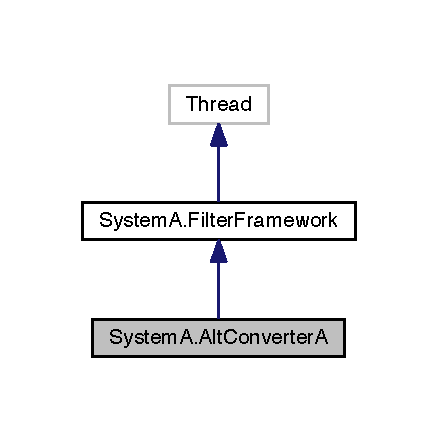
\includegraphics[width=210pt]{class_system_a_1_1_alt_converter_a__inherit__graph}
\end{center}
\end{figure}


Collaboration diagram for System\+A.\+Alt\+Converter\+A\+:\nopagebreak
\begin{figure}[H]
\begin{center}
\leavevmode
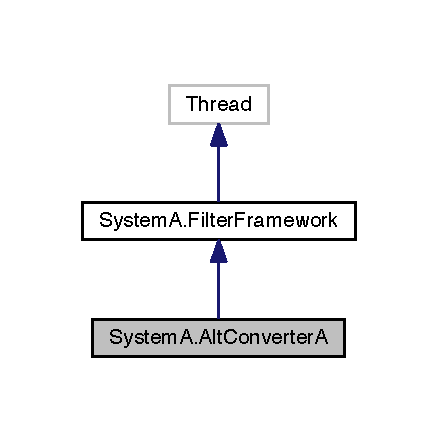
\includegraphics[width=210pt]{class_system_a_1_1_alt_converter_a__coll__graph}
\end{center}
\end{figure}
\subsection*{Public Member Functions}
\begin{DoxyCompactItemize}
\item 
\hyperlink{class_system_a_1_1_alt_converter_a_ad794069151a7712741899c0739cf392a}{Alt\+Converter\+A} (Hash\+Set$<$ Integer $>$ codes\+Set)
\item 
void \hyperlink{class_system_a_1_1_alt_converter_a_a81ea7b005a50a268710ce0ccb89cc754}{run} ()
\end{DoxyCompactItemize}
\subsection*{Additional Inherited Members}


\subsection{Detailed Description}
This is one of the converter filters for System\+A, it takes altitude data and converts from feet to meters, writing the data to the downstream. \begin{DoxyAuthor}{Author}
ligu 
\end{DoxyAuthor}


\subsection{Constructor \& Destructor Documentation}
\hypertarget{class_system_a_1_1_alt_converter_a_ad794069151a7712741899c0739cf392a}{}\index{System\+A\+::\+Alt\+Converter\+A@{System\+A\+::\+Alt\+Converter\+A}!Alt\+Converter\+A@{Alt\+Converter\+A}}
\index{Alt\+Converter\+A@{Alt\+Converter\+A}!System\+A\+::\+Alt\+Converter\+A@{System\+A\+::\+Alt\+Converter\+A}}
\subsubsection[{Alt\+Converter\+A}]{\setlength{\rightskip}{0pt plus 5cm}System\+A.\+Alt\+Converter\+A.\+Alt\+Converter\+A (
\begin{DoxyParamCaption}
\item[{Hash\+Set$<$ Integer $>$}]{codes\+Set}
\end{DoxyParamCaption}
)}\label{class_system_a_1_1_alt_converter_a_ad794069151a7712741899c0739cf392a}
Overload the super class constructor 
\begin{DoxyParams}{Parameters}
{\em codes\+Set} & \\
\hline
\end{DoxyParams}


Here is the call graph for this function\+:\nopagebreak
\begin{figure}[H]
\begin{center}
\leavevmode
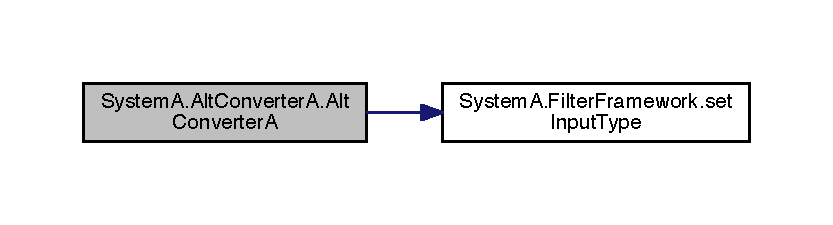
\includegraphics[width=350pt]{class_system_a_1_1_alt_converter_a_ad794069151a7712741899c0739cf392a_cgraph}
\end{center}
\end{figure}




\subsection{Member Function Documentation}
\hypertarget{class_system_a_1_1_alt_converter_a_a81ea7b005a50a268710ce0ccb89cc754}{}\index{System\+A\+::\+Alt\+Converter\+A@{System\+A\+::\+Alt\+Converter\+A}!run@{run}}
\index{run@{run}!System\+A\+::\+Alt\+Converter\+A@{System\+A\+::\+Alt\+Converter\+A}}
\subsubsection[{run}]{\setlength{\rightskip}{0pt plus 5cm}void System\+A.\+Alt\+Converter\+A.\+run (
\begin{DoxyParamCaption}
{}
\end{DoxyParamCaption}
)}\label{class_system_a_1_1_alt_converter_a_a81ea7b005a50a268710ce0ccb89cc754}
Starts off the filter operation Similar to other filters, we read the 4 bytes of I\+D.

If the id is 0, we have time data to write to the output

If the id is 2, we have altitude data. We can simply convert the double from feet to meters Then we fill the measurements byte array with 8 bytes of the altitude in meters so we can write downstream.

The documentation for this class was generated from the following file\+:\begin{DoxyCompactItemize}
\item 
src/\+System\+A/Alt\+Converter\+A.\+java\end{DoxyCompactItemize}

\hypertarget{class_system_a_1_1_filter_framework}{}\section{System\+A.\+Filter\+Framework Class Reference}
\label{class_system_a_1_1_filter_framework}\index{System\+A.\+Filter\+Framework@{System\+A.\+Filter\+Framework}}


Inheritance diagram for System\+A.\+Filter\+Framework\+:
% FIG 0


Collaboration diagram for System\+A.\+Filter\+Framework\+:
% FIG 1
\subsection*{Classes}
\begin{DoxyCompactItemize}
\item 
class {\bfseries End\+Of\+Stream\+Exception}
\end{DoxyCompactItemize}
\subsection*{Public Member Functions}
\begin{DoxyCompactItemize}
\item 
\hyperlink{class_system_a_1_1_filter_framework_ad7ebd0cd900fb578711b6b84079dc80a}{Filter\+Framework} ()
\item 
\hyperlink{class_system_a_1_1_filter_framework_a640d5b39042aa0a66acc3261b03b0434}{Filter\+Framework} (Hash\+Set$<$ Integer $>$ Codes)
\item 
void \hyperlink{class_system_a_1_1_filter_framework_a00efe5c6b5044acdf17db71c297d062e}{run} ()
\item 
\hypertarget{class_system_a_1_1_filter_framework_af98ac10ab07bb2e0e6668590803fc72b}{}Piped\+Input\+Stream {\bfseries get\+Input\+Read\+Port} ()\label{class_system_a_1_1_filter_framework_af98ac10ab07bb2e0e6668590803fc72b}

\item 
\hypertarget{class_system_a_1_1_filter_framework_aae378e5c79852b768d6bd96bd9d0b36e}{}\hyperlink{class_system_a_1_1_filter_framework}{Filter\+Framework} {\bfseries get\+Input\+Filter} ()\label{class_system_a_1_1_filter_framework_aae378e5c79852b768d6bd96bd9d0b36e}

\item 
\hypertarget{class_system_a_1_1_filter_framework_a48f93e54ac19d8208cb42a59e4259b0d}{}void {\bfseries set\+Input\+Filter} (\hyperlink{class_system_a_1_1_filter_framework}{Filter\+Framework} input\+Filter)\label{class_system_a_1_1_filter_framework_a48f93e54ac19d8208cb42a59e4259b0d}

\item 
\hypertarget{class_system_a_1_1_filter_framework_a53f809bc98980394826252ac762cd9e0}{}Piped\+Output\+Stream {\bfseries get\+Output\+Write\+Port} ()\label{class_system_a_1_1_filter_framework_a53f809bc98980394826252ac762cd9e0}

\end{DoxyCompactItemize}
\subsection*{Protected Member Functions}
\begin{DoxyCompactItemize}
\item 
void \hyperlink{class_system_a_1_1_filter_framework_a856b3a8b6b49ad1124de579485e86122}{set\+Input\+Type} (Hash\+Set$<$ Integer $>$ Codes)
\item 
void \hyperlink{class_system_a_1_1_filter_framework_a20e7a6999d87d75474742dafd6edb482}{validate\+Converted\+Codes} (Hash\+Set$<$ Integer $>$ Codes)  throws I\+O\+Exception
\item 
boolean \hyperlink{class_system_a_1_1_filter_framework_ac54511ad34d190b58ea3baecd6a70692}{End\+Of\+Input\+Stream} ()
\end{DoxyCompactItemize}


\subsection{Detailed Description}
\begin{DoxyAuthor}{Author}
ligu Description\+:
\end{DoxyAuthor}
This superclass defines a skeletal filter framework that defines a filter in terms of the input and output ports. All filters must be defined in terms of this framework -\/ that is, filters must extend this class in order to be considered valid system filters. Filters as standalone threads until the inputport no longer has any data -\/ at which point the filter finishes up any work it has to do and then terminates.

Parameters\+:

Input\+Read\+Port\+: This is the filter\textquotesingle{}s input port. Essentially this port is connected to another filter\textquotesingle{}s piped output steam. All filters connect to other filters by connecting their input ports to other filter\textquotesingle{}s output ports. This is handled by the Connect() method.

Output\+Write\+Port\+: This the filter\textquotesingle{}s output port. Essentially the filter\textquotesingle{}s job is to read data from the input port, perform some operation on the data, then write the transformed data on the output port.

\hyperlink{class_system_a_1_1_filter_framework}{Filter\+Framework}\+: This is a reference to the filter that is connected to the instance filter\textquotesingle{}s input port. This reference is to determine when the upstream filter has stopped sending data along the pipe.

converted\+Codes\+: This is a set of integers that represents what kind of inputs the filter is allowed to take. This is a restriction that we took on when we used Acme\+Studio as the architecture builder since every pipe in Acme\+Studio must be coded.

Internal Methods\+:

public void Connect( Filter\+Framework Filter ) public byte Read\+Filter\+Input\+Port() public void Write\+Filter\+Output\+Port(byte datum) public boolean \hyperlink{class_system_a_1_1_filter_framework_ac54511ad34d190b58ea3baecd6a70692}{End\+Of\+Input\+Stream()} protected void \hyperlink{class_system_a_1_1_filter_framework_a856b3a8b6b49ad1124de579485e86122}{set\+Input\+Type(\+Hash\+Set$<$\+Integer$>$ Codes)} protected void \hyperlink{class_system_a_1_1_filter_framework_a20e7a6999d87d75474742dafd6edb482}{validate\+Converted\+Codes(\+Hash\+Set$<$\+Integer$>$ Codes)} 

\subsection{Constructor \& Destructor Documentation}
\hypertarget{class_system_a_1_1_filter_framework_ad7ebd0cd900fb578711b6b84079dc80a}{}\index{System\+A\+::\+Filter\+Framework@{System\+A\+::\+Filter\+Framework}!Filter\+Framework@{Filter\+Framework}}
\index{Filter\+Framework@{Filter\+Framework}!System\+A\+::\+Filter\+Framework@{System\+A\+::\+Filter\+Framework}}
\subsubsection[{Filter\+Framework}]{\setlength{\rightskip}{0pt plus 5cm}System\+A.\+Filter\+Framework.\+Filter\+Framework (
\begin{DoxyParamCaption}
{}
\end{DoxyParamCaption}
)}\label{class_system_a_1_1_filter_framework_ad7ebd0cd900fb578711b6b84079dc80a}
Default constructor \hypertarget{class_system_a_1_1_filter_framework_a640d5b39042aa0a66acc3261b03b0434}{}\index{System\+A\+::\+Filter\+Framework@{System\+A\+::\+Filter\+Framework}!Filter\+Framework@{Filter\+Framework}}
\index{Filter\+Framework@{Filter\+Framework}!System\+A\+::\+Filter\+Framework@{System\+A\+::\+Filter\+Framework}}
\subsubsection[{Filter\+Framework}]{\setlength{\rightskip}{0pt plus 5cm}System\+A.\+Filter\+Framework.\+Filter\+Framework (
\begin{DoxyParamCaption}
\item[{Hash\+Set$<$ Integer $>$}]{Codes}
\end{DoxyParamCaption}
)}\label{class_system_a_1_1_filter_framework_a640d5b39042aa0a66acc3261b03b0434}
Constructor that instantiates a subclass filter with a set of input codes 
\begin{DoxyParams}{Parameters}
{\em Codes} & \\
\hline
\end{DoxyParams}


Here is the call graph for this function\+:
% FIG 2




\subsection{Member Function Documentation}
\hypertarget{class_system_a_1_1_filter_framework_ac54511ad34d190b58ea3baecd6a70692}{}\index{System\+A\+::\+Filter\+Framework@{System\+A\+::\+Filter\+Framework}!End\+Of\+Input\+Stream@{End\+Of\+Input\+Stream}}
\index{End\+Of\+Input\+Stream@{End\+Of\+Input\+Stream}!System\+A\+::\+Filter\+Framework@{System\+A\+::\+Filter\+Framework}}
\subsubsection[{End\+Of\+Input\+Stream}]{\setlength{\rightskip}{0pt plus 5cm}boolean System\+A.\+Filter\+Framework.\+End\+Of\+Input\+Stream (
\begin{DoxyParamCaption}
{}
\end{DoxyParamCaption}
)\hspace{0.3cm}{\ttfamily [protected]}}\label{class_system_a_1_1_filter_framework_ac54511ad34d190b58ea3baecd6a70692}
This method is used within this framework which is why it is private It returns a true when there is no more data to read on the input port of the instance filter. What it really does is to check if the upstream filter is still alive. This is done because Java does not reliably handle broken input pipes and will often continue to read (junk) from a broken input pipe. \begin{DoxyReturn}{Returns}

\end{DoxyReturn}
\hypertarget{class_system_a_1_1_filter_framework_a00efe5c6b5044acdf17db71c297d062e}{}\index{System\+A\+::\+Filter\+Framework@{System\+A\+::\+Filter\+Framework}!run@{run}}
\index{run@{run}!System\+A\+::\+Filter\+Framework@{System\+A\+::\+Filter\+Framework}}
\subsubsection[{run}]{\setlength{\rightskip}{0pt plus 5cm}void System\+A.\+Filter\+Framework.\+run (
\begin{DoxyParamCaption}
{}
\end{DoxyParamCaption}
)}\label{class_system_a_1_1_filter_framework_a00efe5c6b5044acdf17db71c297d062e}
This is actually an abstract method defined by Thread. It is called when the thread is started by calling the Thread.\+start() method. In this case, the \hyperlink{class_system_a_1_1_filter_framework_a00efe5c6b5044acdf17db71c297d062e}{run()} method should be overridden by the filter programmer using this framework superclass \hypertarget{class_system_a_1_1_filter_framework_a856b3a8b6b49ad1124de579485e86122}{}\index{System\+A\+::\+Filter\+Framework@{System\+A\+::\+Filter\+Framework}!set\+Input\+Type@{set\+Input\+Type}}
\index{set\+Input\+Type@{set\+Input\+Type}!System\+A\+::\+Filter\+Framework@{System\+A\+::\+Filter\+Framework}}
\subsubsection[{set\+Input\+Type}]{\setlength{\rightskip}{0pt plus 5cm}void System\+A.\+Filter\+Framework.\+set\+Input\+Type (
\begin{DoxyParamCaption}
\item[{Hash\+Set$<$ Integer $>$}]{Codes}
\end{DoxyParamCaption}
)\hspace{0.3cm}{\ttfamily [protected]}}\label{class_system_a_1_1_filter_framework_a856b3a8b6b49ad1124de579485e86122}
The method used to set the object\textquotesingle{}s input codes 
\begin{DoxyParams}{Parameters}
{\em Codes} & \\
\hline
\end{DoxyParams}


Here is the caller graph for this function\+:
% FIG 3


\hypertarget{class_system_a_1_1_filter_framework_a20e7a6999d87d75474742dafd6edb482}{}\index{System\+A\+::\+Filter\+Framework@{System\+A\+::\+Filter\+Framework}!validate\+Converted\+Codes@{validate\+Converted\+Codes}}
\index{validate\+Converted\+Codes@{validate\+Converted\+Codes}!System\+A\+::\+Filter\+Framework@{System\+A\+::\+Filter\+Framework}}
\subsubsection[{validate\+Converted\+Codes}]{\setlength{\rightskip}{0pt plus 5cm}void System\+A.\+Filter\+Framework.\+validate\+Converted\+Codes (
\begin{DoxyParamCaption}
\item[{Hash\+Set$<$ Integer $>$}]{Codes}
\end{DoxyParamCaption}
) throws I\+O\+Exception\hspace{0.3cm}{\ttfamily [protected]}}\label{class_system_a_1_1_filter_framework_a20e7a6999d87d75474742dafd6edb482}
The method that validates the codes provided with the object\textquotesingle{}s input codes. Every filter being connected to is passed a set of input codes that are then validated using this method. If there are discrepancies, the method throws an exception. This is similar to how Acme\+Studios would raise an error if the codes do not match for filter pipes. 
\begin{DoxyParams}{Parameters}
{\em Codes} & \\
\hline
\end{DoxyParams}

\begin{DoxyExceptions}{Exceptions}
{\em I\+O\+Exception} & \\
\hline
\end{DoxyExceptions}


The documentation for this class was generated from the following file\+:\begin{DoxyCompactItemize}
\item 
src/\+System\+A/Filter\+Framework.\+java\end{DoxyCompactItemize}

\hypertarget{class_system_a_1_1_merge_filter_a}{}\section{System\+A.\+Merge\+Filter\+A Class Reference}
\label{class_system_a_1_1_merge_filter_a}\index{System\+A.\+Merge\+Filter\+A@{System\+A.\+Merge\+Filter\+A}}


Inheritance diagram for System\+A.\+Merge\+Filter\+A\+:
\nopagebreak
\begin{figure}[H]
\begin{center}
\leavevmode
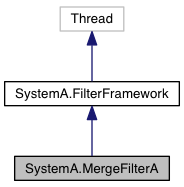
\includegraphics[width=210pt]{class_system_a_1_1_merge_filter_a__inherit__graph}
\end{center}
\end{figure}


Collaboration diagram for System\+A.\+Merge\+Filter\+A\+:
\nopagebreak
\begin{figure}[H]
\begin{center}
\leavevmode
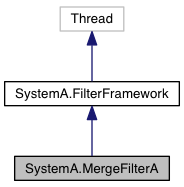
\includegraphics[width=210pt]{class_system_a_1_1_merge_filter_a__coll__graph}
\end{center}
\end{figure}
\subsection*{Public Member Functions}
\begin{DoxyCompactItemize}
\item 
\hyperlink{class_system_a_1_1_merge_filter_a_acdc58d2d95e2a59ff8a6731aa18d7c2d}{Merge\+Filter\+A} (Hash\+Set$<$ Integer $>$ codes\+Set)
\item 
void \hyperlink{class_system_a_1_1_merge_filter_a_acab836dc5b0be101c3da5ab856477172}{run} ()
\item 
\hypertarget{class_system_a_1_1_merge_filter_a_a2448cf368797f26dc1eacf80a1a1ece4}{}Piped\+Input\+Stream {\bfseries get\+Input\+Read\+Port2} ()\label{class_system_a_1_1_merge_filter_a_a2448cf368797f26dc1eacf80a1a1ece4}

\end{DoxyCompactItemize}
\subsection*{Additional Inherited Members}


\subsection{Detailed Description}
This method takes input from both the altitude converter and the temperature converter, merging the inputstreams for the sink filter to write to output. This class is special in that it has T\+W\+O inputports, one in the superclass and one as a private member of the subclass. \begin{DoxyAuthor}{Author}
ligu 
\end{DoxyAuthor}


\subsection{Constructor \& Destructor Documentation}
\hypertarget{class_system_a_1_1_merge_filter_a_acdc58d2d95e2a59ff8a6731aa18d7c2d}{}\index{System\+A\+::\+Merge\+Filter\+A@{System\+A\+::\+Merge\+Filter\+A}!Merge\+Filter\+A@{Merge\+Filter\+A}}
\index{Merge\+Filter\+A@{Merge\+Filter\+A}!System\+A\+::\+Merge\+Filter\+A@{System\+A\+::\+Merge\+Filter\+A}}
\subsubsection[{Merge\+Filter\+A}]{\setlength{\rightskip}{0pt plus 5cm}System\+A.\+Merge\+Filter\+A.\+Merge\+Filter\+A (
\begin{DoxyParamCaption}
\item[{Hash\+Set$<$ Integer $>$}]{codes\+Set}
\end{DoxyParamCaption}
)}\label{class_system_a_1_1_merge_filter_a_acdc58d2d95e2a59ff8a6731aa18d7c2d}
Overload the superclass constructor 
\begin{DoxyParams}{Parameters}
{\em codes\+Set} & \\
\hline
\end{DoxyParams}


Here is the call graph for this function\+:
\nopagebreak
\begin{figure}[H]
\begin{center}
\leavevmode
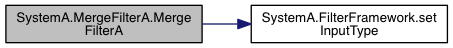
\includegraphics[width=350pt]{class_system_a_1_1_merge_filter_a_acdc58d2d95e2a59ff8a6731aa18d7c2d_cgraph}
\end{center}
\end{figure}




\subsection{Member Function Documentation}
\hypertarget{class_system_a_1_1_merge_filter_a_acab836dc5b0be101c3da5ab856477172}{}\index{System\+A\+::\+Merge\+Filter\+A@{System\+A\+::\+Merge\+Filter\+A}!run@{run}}
\index{run@{run}!System\+A\+::\+Merge\+Filter\+A@{System\+A\+::\+Merge\+Filter\+A}}
\subsubsection[{run}]{\setlength{\rightskip}{0pt plus 5cm}void System\+A.\+Merge\+Filter\+A.\+run (
\begin{DoxyParamCaption}
{}
\end{DoxyParamCaption}
)}\label{class_system_a_1_1_merge_filter_a_acab836dc5b0be101c3da5ab856477172}
Runs the filter Two measurements are taken concurrently, measurement2 is from inputport2, which would be the temperature data. measurement is from inputport1, which would be the altitude data.

Two I\+D\textquotesingle{}s are stored in similar fashion.

Just as we need two byte arrays before, we need four this time.

Read four bytes of I\+D from the second input port

Read four bytes of I\+D from the first input port

Read 8 bytes of measurements from the second input port. Buffering as necessary.

Read 8 bytes of measurements from the first input port. Buffering as necessary.

The only data in id\+\_\+bytes2 and data\+\_\+bytes2 are time and temperature. We want to write them to the output either way.

We O\+N\+L\+Y write I\+D and data from the first inputport if the measurements are altitude. We do not care about the time since the previous write would have covered it.

The documentation for this class was generated from the following file\+:\begin{DoxyCompactItemize}
\item 
src/\+System\+A/Merge\+Filter\+A.\+java\end{DoxyCompactItemize}

\hypertarget{class_system_a_1_1_plumber_a}{}\section{System\+A.\+Plumber\+A Class Reference}
\label{class_system_a_1_1_plumber_a}\index{System\+A.\+Plumber\+A@{System\+A.\+Plumber\+A}}
\subsection*{Static Public Member Functions}
\begin{DoxyCompactItemize}
\item 
static void \hyperlink{class_system_a_1_1_plumber_a_aa3c57a5fc378572e7bbeb475fbe1451d}{main} (String argv\mbox{[}$\,$\mbox{]})  throws I\+O\+Exception 	   
\end{DoxyCompactItemize}


\subsection{Detailed Description}
This class is the Plumber for System\+A. It instantiates all the filter subclasses needed for the first System, each with a set of input codes as defined by the provided architecture. It then connects all the filters and starts them off. \begin{DoxyAuthor}{Author}
ligu 
\end{DoxyAuthor}


\subsection{Member Function Documentation}
\hypertarget{class_system_a_1_1_plumber_a_aa3c57a5fc378572e7bbeb475fbe1451d}{}\index{System\+A\+::\+Plumber\+A@{System\+A\+::\+Plumber\+A}!main@{main}}
\index{main@{main}!System\+A\+::\+Plumber\+A@{System\+A\+::\+Plumber\+A}}
\subsubsection[{main}]{\setlength{\rightskip}{0pt plus 5cm}static void System\+A.\+Plumber\+A.\+main (
\begin{DoxyParamCaption}
\item[{String}]{argv\mbox{[}$\,$\mbox{]}}
\end{DoxyParamCaption}
) throws I\+O\+Exception\hspace{0.3cm}{\ttfamily [static]}}\label{class_system_a_1_1_plumber_a_aa3c57a5fc378572e7bbeb475fbe1451d}
The main method is ran, it starts all the filters off. 
\begin{DoxyParams}{Parameters}
{\em argv} & \\
\hline
\end{DoxyParams}

\begin{DoxyExceptions}{Exceptions}
{\em I\+O\+Exception} & \\
\hline
\end{DoxyExceptions}


The documentation for this class was generated from the following file\+:\begin{DoxyCompactItemize}
\item 
src/\+System\+A/Plumber\+A.\+java\end{DoxyCompactItemize}

\hypertarget{class_system_a_1_1_sink_filter_a}{}\section{System\+A.\+Sink\+Filter\+A Class Reference}
\label{class_system_a_1_1_sink_filter_a}\index{System\+A.\+Sink\+Filter\+A@{System\+A.\+Sink\+Filter\+A}}


Inheritance diagram for System\+A.\+Sink\+Filter\+A\+:\nopagebreak
\begin{figure}[H]
\begin{center}
\leavevmode
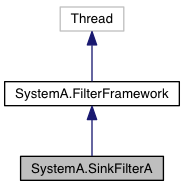
\includegraphics[width=210pt]{class_system_a_1_1_sink_filter_a__inherit__graph}
\end{center}
\end{figure}


Collaboration diagram for System\+A.\+Sink\+Filter\+A\+:\nopagebreak
\begin{figure}[H]
\begin{center}
\leavevmode
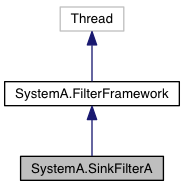
\includegraphics[width=210pt]{class_system_a_1_1_sink_filter_a__coll__graph}
\end{center}
\end{figure}
\subsection*{Public Member Functions}
\begin{DoxyCompactItemize}
\item 
void \hyperlink{class_system_a_1_1_sink_filter_a_a1d101cb86c9cdf2ab9dd8e7e47439e15}{run} ()
\end{DoxyCompactItemize}
\subsection*{Additional Inherited Members}


\subsection{Detailed Description}
This class is the Sink Filter for System\+A. It is the final step in the System\+A process. It takes the upstream data and write them to the outputfile. \begin{DoxyAuthor}{Author}
ligu, Tony 
\end{DoxyAuthor}


\subsection{Member Function Documentation}
\hypertarget{class_system_a_1_1_sink_filter_a_a1d101cb86c9cdf2ab9dd8e7e47439e15}{}\index{System\+A\+::\+Sink\+Filter\+A@{System\+A\+::\+Sink\+Filter\+A}!run@{run}}
\index{run@{run}!System\+A\+::\+Sink\+Filter\+A@{System\+A\+::\+Sink\+Filter\+A}}
\subsubsection[{run}]{\setlength{\rightskip}{0pt plus 5cm}void System\+A.\+Sink\+Filter\+A.\+run (
\begin{DoxyParamCaption}
{}
\end{DoxyParamCaption}
)}\label{class_system_a_1_1_sink_filter_a_a1d101cb86c9cdf2ab9dd8e7e47439e15}
This method runs the sink filter. 

The documentation for this class was generated from the following file\+:\begin{DoxyCompactItemize}
\item 
src/\+System\+A/Sink\+Filter\+A.\+java\end{DoxyCompactItemize}

\hypertarget{class_system_a_1_1_source_filter_a}{}\section{System\+A.\+Source\+Filter\+A Class Reference}
\label{class_system_a_1_1_source_filter_a}\index{System\+A.\+Source\+Filter\+A@{System\+A.\+Source\+Filter\+A}}


Inheritance diagram for System\+A.\+Source\+Filter\+A\+:
\nopagebreak
\begin{figure}[H]
\begin{center}
\leavevmode
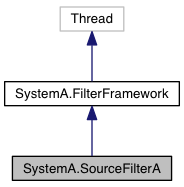
\includegraphics[width=210pt]{class_system_a_1_1_source_filter_a__inherit__graph}
\end{center}
\end{figure}


Collaboration diagram for System\+A.\+Source\+Filter\+A\+:
\nopagebreak
\begin{figure}[H]
\begin{center}
\leavevmode
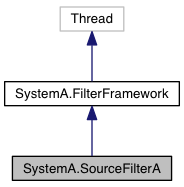
\includegraphics[width=210pt]{class_system_a_1_1_source_filter_a__coll__graph}
\end{center}
\end{figure}
\subsection*{Public Member Functions}
\begin{DoxyCompactItemize}
\item 
\hyperlink{class_system_a_1_1_source_filter_a_a8cca3e9d326c13986c466b5e6dc3c148}{Source\+Filter\+A} (Hash\+Set$<$ Integer $>$ codes\+Set)
\item 
void \hyperlink{class_system_a_1_1_source_filter_a_a8fbf98238a85ec30488c9117819df20b}{run} ()
\end{DoxyCompactItemize}
\subsection*{Additional Inherited Members}


\subsection{Detailed Description}
This class is the Source Filter for System\+A. It does not do much besides read the data from the input file one byte at a time and then send it downstream. \begin{DoxyAuthor}{Author}
ligu, Tony 
\end{DoxyAuthor}


\subsection{Constructor \& Destructor Documentation}
\hypertarget{class_system_a_1_1_source_filter_a_a8cca3e9d326c13986c466b5e6dc3c148}{}\index{System\+A\+::\+Source\+Filter\+A@{System\+A\+::\+Source\+Filter\+A}!Source\+Filter\+A@{Source\+Filter\+A}}
\index{Source\+Filter\+A@{Source\+Filter\+A}!System\+A\+::\+Source\+Filter\+A@{System\+A\+::\+Source\+Filter\+A}}
\subsubsection[{Source\+Filter\+A}]{\setlength{\rightskip}{0pt plus 5cm}System\+A.\+Source\+Filter\+A.\+Source\+Filter\+A (
\begin{DoxyParamCaption}
\item[{Hash\+Set$<$ Integer $>$}]{codes\+Set}
\end{DoxyParamCaption}
)}\label{class_system_a_1_1_source_filter_a_a8cca3e9d326c13986c466b5e6dc3c148}
Overload the superclass constructor. 
\begin{DoxyParams}{Parameters}
{\em codes\+Set} & \\
\hline
\end{DoxyParams}


Here is the call graph for this function\+:
\nopagebreak
\begin{figure}[H]
\begin{center}
\leavevmode
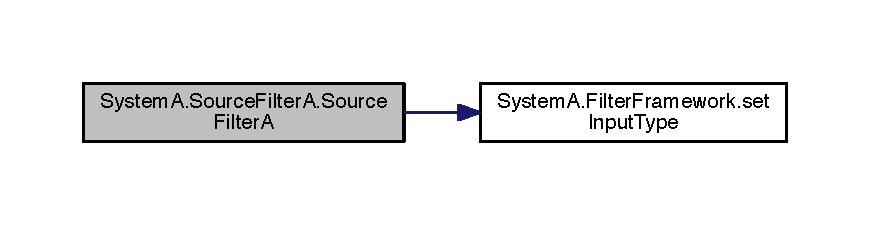
\includegraphics[width=350pt]{class_system_a_1_1_source_filter_a_a8cca3e9d326c13986c466b5e6dc3c148_cgraph}
\end{center}
\end{figure}




\subsection{Member Function Documentation}
\hypertarget{class_system_a_1_1_source_filter_a_a8fbf98238a85ec30488c9117819df20b}{}\index{System\+A\+::\+Source\+Filter\+A@{System\+A\+::\+Source\+Filter\+A}!run@{run}}
\index{run@{run}!System\+A\+::\+Source\+Filter\+A@{System\+A\+::\+Source\+Filter\+A}}
\subsubsection[{run}]{\setlength{\rightskip}{0pt plus 5cm}void System\+A.\+Source\+Filter\+A.\+run (
\begin{DoxyParamCaption}
{}
\end{DoxyParamCaption}
)}\label{class_system_a_1_1_source_filter_a_a8fbf98238a85ec30488c9117819df20b}
This method is the body of the filter. It runs the actual filter operation. 

The documentation for this class was generated from the following file\+:\begin{DoxyCompactItemize}
\item 
src/\+System\+A/Source\+Filter\+A.\+java\end{DoxyCompactItemize}

\hypertarget{class_system_a_1_1_splitter_filter_a}{}\section{System\+A.\+Splitter\+Filter\+A Class Reference}
\label{class_system_a_1_1_splitter_filter_a}\index{System\+A.\+Splitter\+Filter\+A@{System\+A.\+Splitter\+Filter\+A}}


Inheritance diagram for System\+A.\+Splitter\+Filter\+A\+:\nopagebreak
\begin{figure}[H]
\begin{center}
\leavevmode
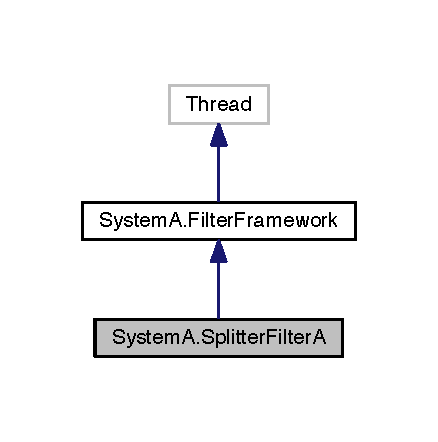
\includegraphics[width=210pt]{class_system_a_1_1_splitter_filter_a__inherit__graph}
\end{center}
\end{figure}


Collaboration diagram for System\+A.\+Splitter\+Filter\+A\+:\nopagebreak
\begin{figure}[H]
\begin{center}
\leavevmode
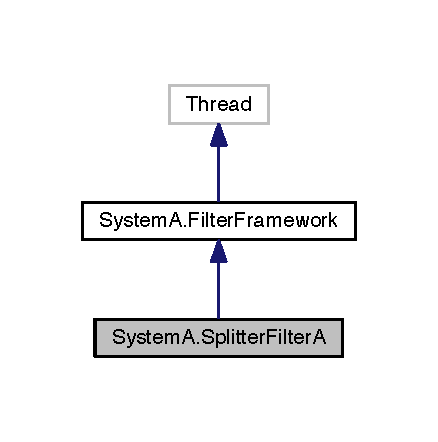
\includegraphics[width=210pt]{class_system_a_1_1_splitter_filter_a__coll__graph}
\end{center}
\end{figure}
\subsection*{Public Member Functions}
\begin{DoxyCompactItemize}
\item 
\hyperlink{class_system_a_1_1_splitter_filter_a_a79dc23af7be9dbb22286bce76cb79c18}{Splitter\+Filter\+A} (Hash\+Set$<$ Integer $>$ codes\+Set)
\item 
void \hyperlink{class_system_a_1_1_splitter_filter_a_a7ce43d0ac6d5aaf0c55f5d4417ec286a}{run} ()
\item 
\hypertarget{class_system_a_1_1_splitter_filter_a_abf1e9e0fb5fe6851c77d7724618cf81f}{}Piped\+Output\+Stream {\bfseries get\+Output\+Write\+Port2} ()\label{class_system_a_1_1_splitter_filter_a_abf1e9e0fb5fe6851c77d7724618cf81f}

\end{DoxyCompactItemize}
\subsection*{Additional Inherited Members}


\subsection{Detailed Description}
This is Splitter\+Filter for System\+A. This one is responsible for taking the raw input stream from the source and split it up. In the case of System\+A, time and altitude go to the Alt\+Converter, time and temperature goto the Temp\+Converter filter. The other data don\textquotesingle{}t go anywhere since we don\textquotesingle{}t care about them in System\+A.

This class is somewhat special. We tried to preserve the original Framework, which is suited to one inputport and one outputport. Since our architecture calls for two outputports, we have to add another private member to this filter. This calls for the overriding of some methods of the superclass and some new methods. \begin{DoxyAuthor}{Author}
ligu 
\end{DoxyAuthor}


\subsection{Constructor \& Destructor Documentation}
\hypertarget{class_system_a_1_1_splitter_filter_a_a79dc23af7be9dbb22286bce76cb79c18}{}\index{System\+A\+::\+Splitter\+Filter\+A@{System\+A\+::\+Splitter\+Filter\+A}!Splitter\+Filter\+A@{Splitter\+Filter\+A}}
\index{Splitter\+Filter\+A@{Splitter\+Filter\+A}!System\+A\+::\+Splitter\+Filter\+A@{System\+A\+::\+Splitter\+Filter\+A}}
\subsubsection[{Splitter\+Filter\+A}]{\setlength{\rightskip}{0pt plus 5cm}System\+A.\+Splitter\+Filter\+A.\+Splitter\+Filter\+A (
\begin{DoxyParamCaption}
\item[{Hash\+Set$<$ Integer $>$}]{codes\+Set}
\end{DoxyParamCaption}
)}\label{class_system_a_1_1_splitter_filter_a_a79dc23af7be9dbb22286bce76cb79c18}
Overload the superclass constructor 
\begin{DoxyParams}{Parameters}
{\em codes\+Set} & \\
\hline
\end{DoxyParams}


Here is the call graph for this function\+:\nopagebreak
\begin{figure}[H]
\begin{center}
\leavevmode
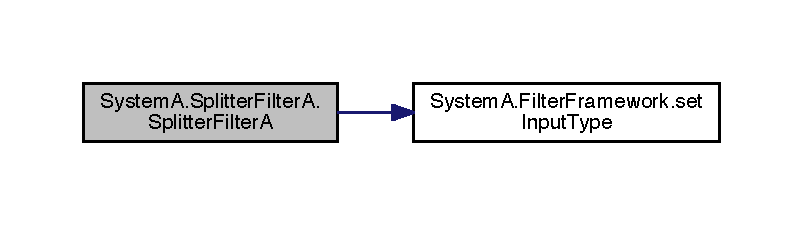
\includegraphics[width=350pt]{class_system_a_1_1_splitter_filter_a_a79dc23af7be9dbb22286bce76cb79c18_cgraph}
\end{center}
\end{figure}




\subsection{Member Function Documentation}
\hypertarget{class_system_a_1_1_splitter_filter_a_a7ce43d0ac6d5aaf0c55f5d4417ec286a}{}\index{System\+A\+::\+Splitter\+Filter\+A@{System\+A\+::\+Splitter\+Filter\+A}!run@{run}}
\index{run@{run}!System\+A\+::\+Splitter\+Filter\+A@{System\+A\+::\+Splitter\+Filter\+A}}
\subsubsection[{run}]{\setlength{\rightskip}{0pt plus 5cm}void System\+A.\+Splitter\+Filter\+A.\+run (
\begin{DoxyParamCaption}
{}
\end{DoxyParamCaption}
)}\label{class_system_a_1_1_splitter_filter_a_a7ce43d0ac6d5aaf0c55f5d4417ec286a}
Starts off the filter. Similar to other filters, we read the 4 bytes of I\+D.

If the id is 0, that means we have time. According to our architecture, time data goes to both of the outputports. So we go through both the id and measurement byte arrays and write to both outputports.

In the case of altitude, we only need to send the data to \hyperlink{class_system_a_1_1_alt_converter_a}{Alt\+Converter\+A}

Where in the case of temperature, it is sufficient to go to \hyperlink{class_system_a_1_1_temp_converter_a}{Temp\+Converter\+A}

The documentation for this class was generated from the following file\+:\begin{DoxyCompactItemize}
\item 
src/\+System\+A/Splitter\+Filter\+A.\+java\end{DoxyCompactItemize}

\hypertarget{class_system_a_1_1_temp_converter_a}{}\section{System\+A.\+Temp\+Converter\+A Class Reference}
\label{class_system_a_1_1_temp_converter_a}\index{System\+A.\+Temp\+Converter\+A@{System\+A.\+Temp\+Converter\+A}}


Inheritance diagram for System\+A.\+Temp\+Converter\+A\+:
\nopagebreak
\begin{figure}[H]
\begin{center}
\leavevmode
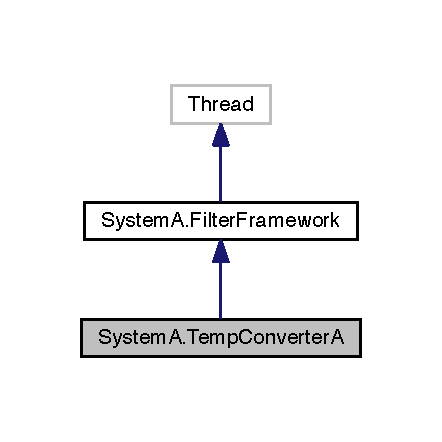
\includegraphics[width=212pt]{class_system_a_1_1_temp_converter_a__inherit__graph}
\end{center}
\end{figure}


Collaboration diagram for System\+A.\+Temp\+Converter\+A\+:
\nopagebreak
\begin{figure}[H]
\begin{center}
\leavevmode
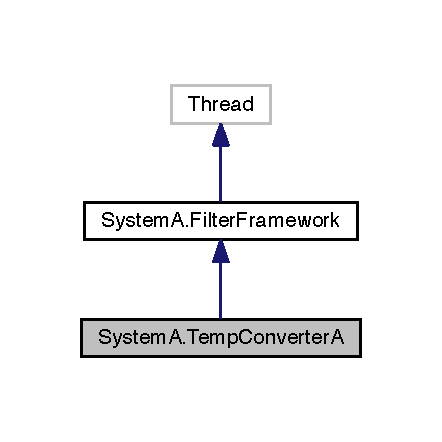
\includegraphics[width=212pt]{class_system_a_1_1_temp_converter_a__coll__graph}
\end{center}
\end{figure}
\subsection*{Public Member Functions}
\begin{DoxyCompactItemize}
\item 
\hyperlink{class_system_a_1_1_temp_converter_a_a7db095a2db61839462d24eb08c00679a}{Temp\+Converter\+A} (Hash\+Set$<$ Integer $>$ codes\+Set)
\item 
void \hyperlink{class_system_a_1_1_temp_converter_a_a12be4f2452c1138c98500526f0d151a4}{run} ()
\end{DoxyCompactItemize}
\subsection*{Additional Inherited Members}


\subsection{Detailed Description}
This is one of the converter filters for System\+A, it takes temperature data and converts from feet to meters, writing the data to the downstream.

This one is a bit different from the altitude converter. Both this one and the altitude converter have the same upstream. In order to make sure that this filter is hooked up to the correct outputport, we have to override the Connect method. \begin{DoxyAuthor}{Author}
ligu 
\end{DoxyAuthor}


\subsection{Constructor \& Destructor Documentation}
\hypertarget{class_system_a_1_1_temp_converter_a_a7db095a2db61839462d24eb08c00679a}{}\index{System\+A\+::\+Temp\+Converter\+A@{System\+A\+::\+Temp\+Converter\+A}!Temp\+Converter\+A@{Temp\+Converter\+A}}
\index{Temp\+Converter\+A@{Temp\+Converter\+A}!System\+A\+::\+Temp\+Converter\+A@{System\+A\+::\+Temp\+Converter\+A}}
\subsubsection[{Temp\+Converter\+A}]{\setlength{\rightskip}{0pt plus 5cm}System\+A.\+Temp\+Converter\+A.\+Temp\+Converter\+A (
\begin{DoxyParamCaption}
\item[{Hash\+Set$<$ Integer $>$}]{codes\+Set}
\end{DoxyParamCaption}
)}\label{class_system_a_1_1_temp_converter_a_a7db095a2db61839462d24eb08c00679a}
Overload the super class constructor 
\begin{DoxyParams}{Parameters}
{\em codes\+Set} & \\
\hline
\end{DoxyParams}


Here is the call graph for this function\+:
\nopagebreak
\begin{figure}[H]
\begin{center}
\leavevmode
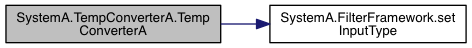
\includegraphics[width=350pt]{class_system_a_1_1_temp_converter_a_a7db095a2db61839462d24eb08c00679a_cgraph}
\end{center}
\end{figure}




\subsection{Member Function Documentation}
\hypertarget{class_system_a_1_1_temp_converter_a_a12be4f2452c1138c98500526f0d151a4}{}\index{System\+A\+::\+Temp\+Converter\+A@{System\+A\+::\+Temp\+Converter\+A}!run@{run}}
\index{run@{run}!System\+A\+::\+Temp\+Converter\+A@{System\+A\+::\+Temp\+Converter\+A}}
\subsubsection[{run}]{\setlength{\rightskip}{0pt plus 5cm}void System\+A.\+Temp\+Converter\+A.\+run (
\begin{DoxyParamCaption}
{}
\end{DoxyParamCaption}
)}\label{class_system_a_1_1_temp_converter_a_a12be4f2452c1138c98500526f0d151a4}
Starts off the filter operation Similar to other filters, we read the 4 bytes of I\+D.

If the id is 0, we have time data to write to the output

If the id is 3, we have temperature data. We can simply convert the double from F to C Then we fill the measurements byte array with 8 bytes of the temperature in C so we can write downstream.

The documentation for this class was generated from the following file\+:\begin{DoxyCompactItemize}
\item 
src/\+System\+A/Temp\+Converter\+A.\+java\end{DoxyCompactItemize}

%--- End generated contents ---

% Index
\backmatter
\newpage
\phantomsection
\clearemptydoublepage
\addcontentsline{toc}{chapter}{Index}
\printindex

\end{document}
